\section{Heterogenius y el 'Arbol de An'alisis}

El 'arbol de an'alisis de Heterogenius es el elemento principal de un proceso de demostraci'on. Es donde se realizan todas las acciones y es donde se refleja el camino tomado para lograr una demostraci'on exitosa. Cada nodo del 'arbol representa un secuente en alg'un lenguaje soportado por Heterogenius. Las aristas corresponden con las acciones ejecutadas. Dependiendo del lenguaje en el que est'e el secuente se habilitan diferentes acciones, pero en general se las puede dividir en tres categor'ias:

\begin{itemize}
\label{clasificacion}
\item las de c'alculo de secuentes, son acciones que transforman un secuente en otro. Algunas pueden producir multiples secuentes (por ejemplo la acci'on \textit{Case}) creando varias ramas que tienen que ser demostradas para lograr un resultado en el nodo raiz.

\item las acciones de traducci'on, traducen un secuente de un lenguaje a otro. Dependiendo de la expresividad del lenguaje esta traducci'on puede ser con perdida o no.

\item las acciones de b'usqueda de contraejemplos, implican el uso de herramientas externas para buscar contraejemplos en el secuente donde se aplique la acci'on. El resultado puede ser positivo, se encontr'o un contraejemplo o negativo, no se encontr'o nada pero 'esto no nos dice nada de la existencia del contraejemplo.
\end{itemize}

\subsection{Limitaciones}

En su versi'on actual, Heterogenius presenta varios problemas y limitaciones. A continuaci'on se detallar'an algunas de 'estas limitaciones que fueron tratadas en 'esta tesis:

Lo primero que se puede notar es la falta de \textit{heterogeneidad verdadera}. Si bien Heterogenius permite realizar una demostraci'on en diferentes lenguajes, cada secuente se limita a tener un solo lenguaje. Debido a 'esto se puede decir que Heterogenius, en realidad permite tener demostraciones heterogeneas con secuentes homogeneos. 

Otro gran problema con el que nos encontramos es la incapacidad del 'arbol de an'alisis de documentar el proceso de an'alisis completo. O sea, el 'arbol solamente muestra las acciones y pasos que llevan al 'exito de una demostraci'on. En el momento del an'alisis cuando una rama no lleva al resultado deseado y se quiere probar otro tipo de acciones, es necesario borrar la rama que no di'o resultado. 'Esto lleva a que se pierdan partes del an'alisis que pueden ser 'utiles ya que documentan las acciones probadas (y que no dieron un resultado deseado) y no nos permite tener un historial de todo lo que se hizo en el an'alisis.

El 'arbol de an'alisis tiene solamente un tipo de ramas, que representan acciones obligatorias que se tienen que llevar a cabo para que el resultado se propague al nodo raiz. 'Esto limita la posibilidad de realizar demostraciones alternativas y experimentar en una demostraci'on con diferentes tipos de herramientas, acciones, etc.

Debido a que las herramientas autom'aticas no siempre producen un resultado, decidimos que es necesario tambi'en documentar la aplicaci'on de las acciones a'un si no tienen un resultado definido.   Todo 'esto aporta al objetivo general de documentar todas las acciones realizadas durante el an'alisis.


\section{Rediseño del 'Arbol de An'alisis}

Para solucionar las limitaciones presentadas nos propusimos a rediseñar el 'arbol de an'alisis.

El primer cambio que realizamos es la implementaci'on de \textit{heterogeneidad verdadera}.
Para lograr 'esto flexibilizamos los secuentes permitiendo que tambi'en sean heterogeneos. 'Esto nos permite manejar las demostraciones con mayor flexibilidad y abstraernos a'un m'as del lenguaje usado para describir el problema. La implementaci'on y fundamentos te'oricos se explican con mayor detalle en la secci'on \hyperref[sec:heterogeneidad-verdadera]{\ref*{sec:heterogeneidad-verdadera} }.

En el 'arbol de an'alisis 'este cambio se va a reflejar en la visualizaci'on de los nodos. Los nodos con secuentes heterogeneos van a estar marcados por una \textit{H} y los nodos homogeneos quedar'an sin ninguna marca.

\begin{figure}[H]
	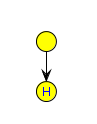
\includegraphics[width=50px]{img/hetero_homo.png}
	\centering
	\caption{El nodo con H contiene un secuente heterog'eneo. El otro nodo es homog'eneo.}
\end{figure}

Para permitir la documentaci'on y el historial de todas las acciones aplicadas asi como la creaci'on de caminos de an'alisis alternativos introdujimos el concepto de \textit{ramificaci'on alternativa}:


\subsection{Ramas alternativas}

Las ramas alternativas representan la existencia de multiples caminos en los que se subdivide el an'alisis para lograr un resultado.. En la interface de Heterogenius 'este tipo de ramas, se representa con lineas punteadas y su significado sem'antico es el de un operador l'ogico \textbf{``o''}. Se corresponde con un camino alternativo en una demostraci'on.

\begin{figure}[H]
	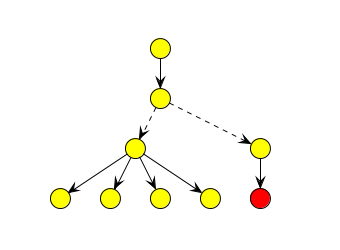
\includegraphics[width=180px]{img/ramas_alternativas_2.png}
	\centering
	\caption{La segunda rama alternativa presenta un contraejemplo. 'Esto indica que existe un contraejemplo para el nodo del cual salen las ramas alternativas.}
\end{figure}

Un nodo con hijos conectados por las ramas alternativas, se entiende que vale si \textit{\textbf{alguna}} de las ramas valen. 'Esto es diferente de la ramificaci'on normal (lineas continuas) que indica que el nodo padre vale si todos sus hijos valen.

Al aplicar una ramificaci'on alternativa a un nodo del 'arbol de an'alisis, el nodo es copiado y agregado como sus propios hijos. 'Esto nos permite trabajar sobre las copias del nodo original. Cuando es necesario tambi'en se puede agregar ramas alternativas durante un an'alisis.
 
La principal ventaja de usar caminos alternativos es la de poder documentar todo el an'alisis que se hizo y las decisiones tomadas, incluso las decisiones que no llevaron al cumplimiento del objetivo. Por otro lado tambi'en nos permite experimentar con diferentes formas de probar lo mismo.

\begin{figure}[H]
	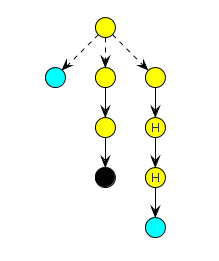
\includegraphics[width=100px]{img/ramas_alternativas.png}
	\centering
	\caption{Tres ramas alternativas: la primera y la 'ultima indican que no se encontr'o ning'un contraejemplo. La segunda rama muestra que se pudo demostrar que el secuente vale, por lo cu'al el secuente del nodo raiz tambi'en vale.}
\end{figure}


\subsection{Nueva Clasificaci'on de Acciones}

Debido a que la clasificaci'on original de las acciones (\ref{clasificacion}) es poco general, propusimos cambiar las categorias para permitir una mayor flexibilidad a la hora de agregar herramientas autom'aticas y acciones nuevas.

La nueva clasificaci'on propuesta es:

\begin{itemize}
\item Acciones de c'alculo de secuentes: son todas las acciones que toman un secuente como su entrada y devuelven uno o mas secuentes. Algunas de 'estas acciones son: \textit{Use}, \textit{Lemma}, \textit{Case}, \textit{Skolem}, etc.

\item Acciones de herramientas estructurales: son acciones que trabajan directamente sobre la estructura del 'arbol de an'alisis. Los traductores-$\rho$ forman parte de 'este grupo, asi como las nuevas acciones introducidas: \textit{carga de antecedentes externos}, \textit{traducci'on-$\rho$ de f'ormulas} y \textit{proyecci'on de f'ormulas}.

\item Acciones de herramientas automaticas: 'este grupo representa a las acciones para las que se usan herramientas autom'aticas como lo son los demostradores autom'aticos de teoremas y los buscadores de contraejemplos.
\end{itemize}

'Esta clasificaci'on se refleja en la arquitectura de Heterogenius y permite guiar las futuras extensiones y funcionalidades adicionales.